% !TeX program = xelatex
% !TeX encoding = UTF-8
% !BIB program = biber
\documentclass[a4paper,oneside,10pt,ngerman,english]{scrbook}

\usepackage[bathesis,fancyfonts]{jkureport}
\usepackage{csquotes}
\usepackage[
  backend=biber,
  style=authoryear,
  natbib=true,
  maxcitenames=2,
  maxbibnames=99,
  uniquename=false,
  doi=true,
  url=true,
  isbn=false
]{biblatex}
\usepackage{amsmath}
\usepackage{booktabs}
\usepackage{graphicx}
\usepackage{xcolor}
\usepackage{enumitem}
\usepackage{listings}
\usepackage{tabularx}

\graphicspath{{figures/}}
\addbibresource{references.bib}

\newcommand{\modelname}{latent Transformer}
\newcommand{\code}[1]{\texttt{#1}}

\begin{document}
\frontmatter

\title{Latent Time-Series Surrogates for Five-Dimensional Gyrokinetic Plasma Turbulence}
\titleshort{Latent Surrogates for Gyrokinetic Turbulence}
\author{Volodymyr~Yelisieiev\matno{12340334}}
\supervisor{Gianluca Galletti}
\degree{Bachelor of Science}{Artificial Intelligence (033 536)}
\submissiondepartment{Institute for Machine Learning}
\date{2026-07-15}
\keywords{gyrokinetics, latent dynamics, Transformer, JAX}
\maketitle

\cleardoubleoddpage
\begin{otherlanguage}{english}
\begin{abstract*}
Gyrokinetic plasma-turbulence simulations are computationally demanding. This thesis tests a
compact latent surrogate for eight-step forecasts of scalar flux and two one-dimensional spectra. A
JAX/Flax pipeline encodes preprocessed snapshots as 128-dimensional states; gated recurrent unit
(GRU) and causal Transformer models roll them forward through frozen diagnostic heads.

The study evaluates 51 trajectories by retrospective five-fold nested group cross-validation with
matched training seeds 52, 53, 54, 55, and 56; it is not a pristine locked-test result. Inner
validation selected Transformer in outer folds 0, 1, and 3 and GRU in folds 2 and 4. The selected
learned models achieved flux root mean squared error (RMSE) 14.6729, versus 10.0207 for copying the
last observed flux across the horizon. The difference was +4.6522 with paired hierarchical-bootstrap
interval [+2.5788, +6.6470]; learned error was lower in 31.6\% of hierarchically weighted paired
runs. The strictly positive interval supports a bounded negative result: the learned models do not
beat observed persistence.

Holding the last latent state fixed and decoding it gave flux RMSE 14.8049. Learned latent mean
squared error (MSE) was 0.4497 versus 0.4307 for latent persistence, a difference of +0.0189 with
interval [-0.0699, +0.1332]. Because this interval includes zero, no latent-dynamics advantage is
established. A diagnostic-head oracle given true future latents reached flux RMSE 12.3732, showing
usable diagnostic information but insufficient accuracy relative to observed persistence; it
isolates no single causal bottleneck.

The contribution is an auditable workflow, not a positive performance claim. Its scope is this
universe, preprocessing, and horizon; it establishes no full-field or long-horizon accuracy,
physical-unit or solver-level performance, broad generalization, a matched numerical comparison with
GyroSwin, or a universal architecture winner.
\end{abstract*}
\end{otherlanguage}

\cleardoubleoddpage
\begin{otherlanguage}{ngerman}
\begin{abstract*}
Gyrokinetische Simulationen von Plasmaturbulenz sind rechenintensiv. Diese Arbeit untersucht,
ob ein kompaktes latentes Ersatzmodell den skalaren Fluss und zwei eindimensionale Spektren über
acht Schritte vorhersagen kann. Eine JAX/Flax-Pipeline kodiert vorverarbeitete Momentaufnahmen als
128-dimensionale Zustände; GRU-Modelle (Gated Recurrent Units) und kausale Transformer-Modelle sagen
deren zeitliche Entwicklung voraus, und eingefrorene Diagnoseköpfe dekodieren die Zielgrößen.

Die Studie wertet 51 Trajektorien mittels retrospektiver fünffacher verschachtelter
Gruppen-Kreuzvalidierung mit denselben Trainings-Seeds 52, 53, 54, 55 und 56 aus; sie ist kein
Ergebnis einer bis zur Auswertung unangetasteten Testmenge. Die innere Validierung wählte den
Transformer in den äußeren Falten 0, 1 und 3 und das GRU-Modell in den Falten 2 und 4. Die
ausgewählten gelernten Modelle erreichten einen Fluss-RMSE (Wurzel des mittleren quadratischen
Fehlers) von 14.6729, während das Fortschreiben des letzten beobachteten Flusswerts über den
Horizont 10.0207 ergab. Die Differenz betrug +4.6522; das gepaarte hierarchische Bootstrap-Intervall
war [+2.5788, +6.6470]. In 31.6\% der hierarchisch gewichteten gepaarten Läufe war der Fehler des
gelernten Modells geringer. Das strikt positive Intervall stützt einen klar begrenzten negativen
Befund: Die gelernten Modelle übertreffen die beobachtete Persistenz nicht.

Das Festhalten am letzten latenten Zustand ergab nach der Dekodierung einen Fluss-RMSE von
14.8049. Der mittlere quadratische Fehler (MSE) im latenten Raum betrug 0.4497 für die gelernten
Modelle und 0.4307 für die latente Persistenz, entsprechend einer Differenz von +0.0189 mit dem
Intervall [-0.0699, +0.1332]. Da dieses Intervall Null einschließt, ist kein Vorteil der gelernten
latenten Dynamik belegt. Eine Oracle-Auswertung, bei der der Diagnosekopf die wahren zukünftigen
latenten Zustände erhielt, erreichte einen Fluss-RMSE von 12.3732. Dies zeigt, dass die Repräsentation
nutzbare diagnostische Informationen enthält, gegenüber der beobachteten Persistenz aber nicht genau
genug ist; einen einzelnen kausalen Engpass isoliert die Oracle-Auswertung nicht.

Der Beitrag liegt in einem überprüfbaren Arbeitsablauf, nicht in einem positiven Leistungsnachweis.
Seine Aussagekraft ist auf dieses Universum, diese Vorverarbeitung und diesen Horizont begrenzt; er
belegt weder vollständige Feld- oder Langzeitgenauigkeit noch Genauigkeit in physikalischen
Einheiten, Solver-Leistung, breite Verallgemeinerung, einen abgestimmten numerischen Vergleich mit
GyroSwin oder die allgemeingültige Überlegenheit einer Architektur.
\end{abstract*}
\end{otherlanguage}


\cleardoubleoddpage
\tableofcontents
\cleardoubleoddpage
\listoffigures
\cleardoubleoddpage
\listoftables

\mainmatter
\cleardoubleoddpage
\chapter{Introduction}
\label{chap:introduction}

\section{Motivation}

Magnetically confined fusion plasmas exhibit turbulence that transports heat and particles across
magnetic surfaces. Predicting this transport is important for understanding confinement, designing
experiments, and deciding which reduced models are safe to use. Nonlinear gyrokinetic equations
retain kinetic effects that fluid approximations can omit, but they evolve a distribution function
over several spatial and velocity coordinates. The resulting five-dimensional state is expensive to
advance at high fidelity, and a long simulation produces a large sequence of strongly correlated
snapshots \citep{abel2013multiscale,paischer2025gyroswin}.

The computational cost creates an attractive role for learned surrogates. A surrogate could provide
fast approximate diagnostics between expensive solver calls, help explore parameter settings, or
serve as a proposal model for a larger simulation workflow. These applications require more than a
low training loss. The model must preserve the information needed by a physical diagnostic, respect
the temporal ordering of trajectories, and be compared with a baseline that is meaningful for the
quantity of interest. If those conditions are not met, a visually smooth rollout can be less useful
than copying the last observed diagnostic.

This thesis studies a deliberately narrow version of that problem. Rather than reconstructing the
complete distribution function, it asks whether a snapshot can be compressed into a small latent
state whose temporal dynamics are easier to learn while still supporting scalar-flux and spectral
diagnostics. Let $x_t$ denote a preprocessed channel-first snapshot, $z_t=f_\theta(x_t)$ its
latent representation, and $g_\phi$ the diagnostic heads. A temporal model $h_\psi$ predicts future
states from a context window. The complete prediction route is therefore
\begin{equation}
  x_{t-L+1:t}\;\xrightarrow{f_\theta}\;z_{t-L+1:t}
  \xrightarrow{h_\psi}\widehat{z}_{t+1:t+H}
  \xrightarrow{g_\phi}\widehat{y}_{t+1:t+H},
\end{equation}
where $y$ contains flux and spectra. The route separates representation learning, temporal
prediction, and diagnostic decoding so that each source of error can be inspected.

This separation has practical advantages. Sequence models operate on vectors rather than a full
spatial grid, so their memory use is easier to control. Diagnostic heads make it possible to test
whether a latent state retains task-relevant information without pretending that it is a complete
physical field. A cached representation also allows persistence, GRU, and Transformer baselines to
share exactly the same encoder and target normalization. The trade-off is equally important: a
latent state is useful only for the information it retains. A small latent MSE does not imply an
accurate transport forecast, and an accurate scalar diagnostic does not imply full-field fidelity.

\section{Why Evaluation Design Matters}

Trajectory data make leakage easy to introduce. Adjacent snapshots from one trajectory are highly
correlated, and a random snapshot split can place near-duplicates in training and evaluation. More
subtly, an encoder trained with one trajectory split can be combined with a sequence evaluator
using another split. The downstream evaluator may call a trajectory ``test'' even though its
snapshots already influenced the encoder or latent normalization. The resulting number can be
finite and reproducible while failing to measure end-to-end generalization.

The thesis therefore treats provenance as part of the experiment, not as an appendix. A manifest
binds the ordered trajectory universe and each outer fold. Resolved configurations record data and
training seeds, normalization scope, context, horizon, and upstream artifact hashes. Validation
selects checkpoints and model families; outer-test evidence is opened only after the selection
barrier. A direct observed-flux persistence baseline is declared before comparison because the
scientific question is diagnostic prediction, not merely latent reconstruction. This design makes
a negative result interpretable: if a learned model loses to persistence, the loss is not hidden by
a weaker reference or by test-aware tuning.

\section{Research Question}

The central research question is:

\begin{quote}
Can a compact JAX/Flax latent surrogate learn short-horizon gyrokinetic dynamics from
preprocessed five-dimensional field snapshots, and do latent sequence models improve
flux-predictive rollouts over direct persistence of the observed flux on held-out trajectories?
\end{quote}

The phrase ``held-out'' is used at the outer-fold level. Because the 51-trajectory universe was
available during development, the final estimate is retrospective nested group cross-validation,
not a pristine locked test. Three sub-questions make the central question measurable:

\begin{enumerate}[label=RQ\arabic*]
  \item Does the encoder retain enough diagnostic signal in a 128-dimensional state for finite
        flux and spectral prediction?
  \item After validation-only checkpoint and family selection, does the selected learned sequence
        model beat direct persistence of the observed flux over an eight-step horizon?
  \item Is any apparent learned-model advantage stable across matched training seeds and outer
        folds, or does the selected family change with the split?
\end{enumerate}

Flux RMSE is the primary metric because transport prediction is the stated goal. Latent MSE,
flux MAE, spectra errors, shape correlation, and finite-output stability are secondary diagnostics.
The hierarchy is intentional: a model that predicts a latent vector well but decodes a poor flux is
not a successful answer to the central question.

\section{Contributions}

This thesis makes the following contributions:

\begin{itemize}
  \item a portable JAX/Flax implementation of a latent-surrogate workflow, including synthetic
        fixtures and a real Cyclone/KvikIO data adapter;
  \item an explicit channel-first tensor contract for five spatial dimensions and deterministic
        trajectory-level split manifests;
  \item a representation objective combining SimSiam-style consistency with supervised flux and
        spectra heads;
  \item latent caching and comparable latent-state persistence, GRU, and causal Transformer
        candidates;
  \item trajectory-balanced rollout evaluation with paired hierarchical uncertainty and separate
        spectral diagnostics;
  \item a frozen five-fold, five-seed evidence record with 230 accepted and 25 skipped stage slots;
        and
  \item a reproducibility-oriented CLI, configuration system, test suite, and release manifest
        that make the negative result auditable without publishing raw data or private paths.
\end{itemize}

The empirical contribution is deliberately bounded. The accepted result shows that the selected
latent models do not beat observed-flux persistence under the declared data and horizon. It does
not establish that latent surrogates are unsuitable for gyrokinetics, nor does it compare numerical
performance with GyroSwin. The software and protocol provide a controlled basis for that future
question.

\section{Scope and Claim Boundaries}

The work predicts latent vectors and diagnostics; it does not reconstruct the complete
five-dimensional state. The medium universe contains 51 trajectories from one preprocessing
pipeline, and the retrospective outer folds provide ten or eleven test trajectories each. The
eight-step horizon establishes short-term behaviour only. Generalization to other regimes,
machines, preprocessing choices, or substantially longer horizons is not established.

GyroSwin is discussed as related work because it targets scalable full-field five-dimensional
surrogacy \citep{paischer2025gyroswin}. A direct numeric comparison is intentionally omitted. Such
a comparison would require the same dataset revision, trajectory split, temporal sampling,
forecast horizon, target definition, normalization, checkpoint, and metric implementation. Without
that matched bundle, a table of numbers would be misleading rather than informative.

\section{Thesis Structure}

\autoref{chap:background} introduces gyrokinetic turbulence, representation learning, and latent
sequence models. \autoref{chap:method} defines the data contract, objectives, architectures, and
evaluation protocol. \autoref{chap:implementation} describes the software system and portability
decisions. \autoref{chap:experiments} specifies the byte-verified universe, nested folds, models,
metrics, and provenance rules. Results are reported in \autoref{chap:results}, interpreted in
\autoref{chap:discussion}, and summarized in \autoref{chap:conclusion}. The required story summary
and reproducibility details are provided in the appendices.

\cleardoubleoddpage
\chapter{Background and Related Work}
\label{chap:background}

\section{Gyrokinetic Turbulence}

Gyrokinetic theory reduces the six-dimensional kinetic description by averaging over the fast
gyromotion while retaining three spatial and two velocity-space coordinates. The resulting
five-dimensional distribution function still supports nonlinear turbulence, scale interactions,
and transport. A complete derivation is outside the scope of this thesis; the multiscale framework
of \citet{abel2013multiscale} provides the physical context. For machine learning, the important
consequence is the size and anisotropy of each state: a snapshot is not a conventional two- or
three-dimensional image, and each axis has a distinct physical interpretation.

The data used here provide the distribution-function field together with a scalar flux target and
two one-dimensional spectra, denoted \code{kyspec} and \code{fluxspec}. Flux summarizes a central
transport quantity, whereas spectra expose some scale-dependent structure. They are therefore
treated as diagnostic targets rather than attempting a full reconstruction of $x_t$.

\section{Neural Surrogates for Gyrokinetics}

Recent work has begun to apply neural surrogates directly to gyrokinetic simulations. GyroSwin
extends hierarchical vision Transformers to five-dimensional fields and couples distribution and
potential representations through specialized modules \citep{paischer2025gyroswin}. Its ambition
is full-field surrogacy and physically verifiable transport estimates. GKFieldFlow instead models
three-dimensional potential fields with a spatial encoder--decoder and temporal convolutions
\citep{ashourvan2026gkfieldflow}. These systems motivate learning temporal structure but solve a
different prediction problem from the compact diagnostic-preserving latent model studied here.

The distinction matters for evaluation. A full-field model may be assessed through reconstruction,
spectral fidelity, and transport diagnostics. This thesis has no decoder and therefore makes no
full-field reconstruction claim. Its strongest evidence is an internal comparison among sequence
models that share one encoder, latent cache, split, and rollout protocol.

Neural-surrogate comparisons also require a baseline that reflects the temporal regularity of the
data. Persistence is particularly demanding when adjacent states change slowly: a learned model
must improve on copying the latest observation, not merely achieve a small absolute error. Model
choice must be separated from final assessment as well. Validation trajectories support choices
such as architecture and normalization, whereas test trajectories estimate performance only after
those choices are fixed. If representation learning has already observed a downstream test
trajectory, the complete surrogate is not held out even when the temporal model itself has not
trained on that trajectory. Model selection and performance estimation must also remain separated:
optimizing a noisy validation criterion can otherwise produce selection bias
\citep{varma2006crossvalidation,cawley2010selectionbias}. These principles motivate the trajectory-level lineage checks and the
validation-then-test protocol used in this thesis.

\section{Self-Supervised Representation Learning}

Representation learning seeks a mapping $f_\theta(x)=z$ that retains useful information while
discarding nuisance variation. Contrastive approaches often compare positive and negative pairs.
SimSiam shows that a Siamese architecture can learn without negative pairs or a momentum encoder,
provided a predictor and stop-gradient operation prevent trivial collapse
\citep{chen2021simsiam}. Given two augmented views $x^{(1)}$ and $x^{(2)}$, the shared encoder and
projection head produce $p_1$ and $p_2$, while a prediction head produces $q_1$ and $q_2$. A
symmetric negative cosine objective aligns each prediction with the stopped projection of the
other view.

PCA gives a linear projection for inspecting broad variance structure, while t-SNE constructs a
nonlinear neighbourhood-preserving visualization \citep{vandermaaten2008tsne}. Neither method is a
forecast metric: apparent clusters or gradients can depend on scaling and projection parameters.
They are therefore used only for descriptive inspection in this work.

Scientific data require conservative augmentations. Transformations that are harmless for natural
images can alter physical meaning. The present implementation uses small additive noise, amplitude
jitter, and sparse element masking. It does not use arbitrary crops or rotations. The
self-supervised objective is combined with flux and spectra supervision so the latent space is
explicitly encouraged to retain the selected diagnostics.

\section{Latent Dynamics Models}

Once snapshots are embedded, the temporal problem becomes vector sequence prediction. Persistence
copies the final context vector and provides a parameter-free baseline. An MLP-delta model predicts
a residual from the flattened context. GRUs use learned gates to update a recurrent state and are a
compact recurrent baseline \citep{cho2014gru}. Transformers replace recurrence with self-attention
over the context \citep{vaswani2017attention}. A causal mask prevents a token from accessing future
positions, and the final token representation predicts the next latent.

Autoregressive rollout introduces distribution shift: the first prediction is conditioned on true
context, whereas later predictions are conditioned partly on previous model outputs. Consequently,
one-step training loss alone does not establish rollout quality. This thesis evaluates recursive
eight-step predictions and reports each horizon as well as aggregated metrics.

\section{Scientific Machine-Learning Stack}

JAX provides accelerator-oriented array computation together with transformations for automatic
differentiation, compilation, vectorization, and device parallelism \citep{jax2026}. Flax supplies
the neural-network module abstraction used here, and Optax supplies composable optimization
updates \citep{flax2026,optax2026}. The implementation uses pure JAX computation at the model and
training boundary, while Python, NumPy, HDF5, and KvikIO-compatible readers handle file I/O. This
division keeps I/O outside compiled functions and permits CPU smoke tests alongside GPU training.

\cleardoubleoddpage
\chapter{Method}
\label{chap:method}

\section{Pipeline Overview}

\autoref{fig:pipeline} summarizes the proposed two-stage surrogate. The encoder is trained first and
then frozen. It converts every trajectory into a latent cache. Sequence models are trained only on
windows from this cache. During evaluation, predicted latents are passed through the frozen
diagnostic heads so that temporal errors can be measured in flux and spectra space.

\begin{figure}[htbp]
  \centering
  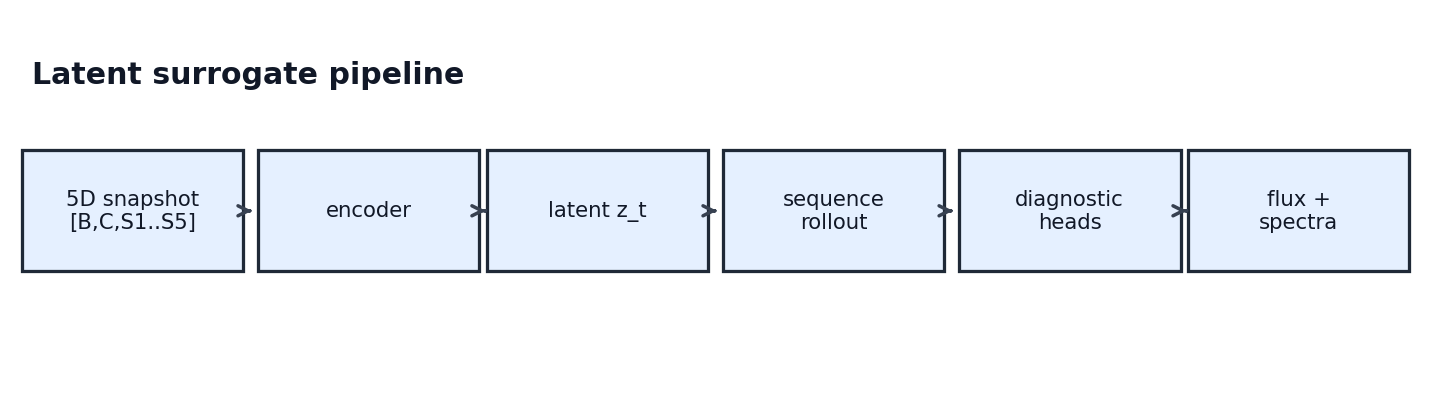
\includegraphics[width=0.95\textwidth]{pipeline_diagram.png}
  \caption{Latent-surrogate pipeline. A five-dimensional snapshot is embedded into a compact
  vector, evolved autoregressively, and evaluated through latent and diagnostic metrics.}
  \label{fig:pipeline}
\end{figure}

This staged design prevents file layout and spatial tensor size from leaking into the sequence
model. It also guarantees that all temporal baselines in a comparison use the same representation.

\section{Data Contract and Splitting}

A single snapshot has shape
\begin{equation}
  x_t \in \mathbb{R}^{C\times S_1\times S_2\times S_3\times S_4\times S_5},
\end{equation}
and a batch has shape
\begin{equation}
  X \in \mathbb{R}^{B\times C\times S_1\times S_2\times S_3\times S_4\times S_5}.
\end{equation}
The validated Cyclone snapshot shape is $(4,32,8,16,85,32)$ before batching. All adapters convert
samples to \code{float32} at the model boundary. The channel-first contract is validated rather
than inferred, because an unnoticed axis permutation would still be numerically executable but
scientifically invalid.

The Cyclone adapter loads a field snapshot at raw index $r$ and attaches flux and spectra from
$r+b$, where the configured bundle offset is $b=1$. Retained field snapshots are separated by the
subsampling stride of eight raw indices. Consequently, the diagnostic head learns
$z(r)\mapsto y(r+1)$, and the diagnostic reported for rollout horizon $h$ corresponds to the target
attached to the predicted retained state, $y(r+8h+1)$. Throughout the thesis, ``flux at horizon
$h$'' refers to this attached diagnostic target rather than a value at exactly the field index.

\begin{figure}[htbp]
  \centering
  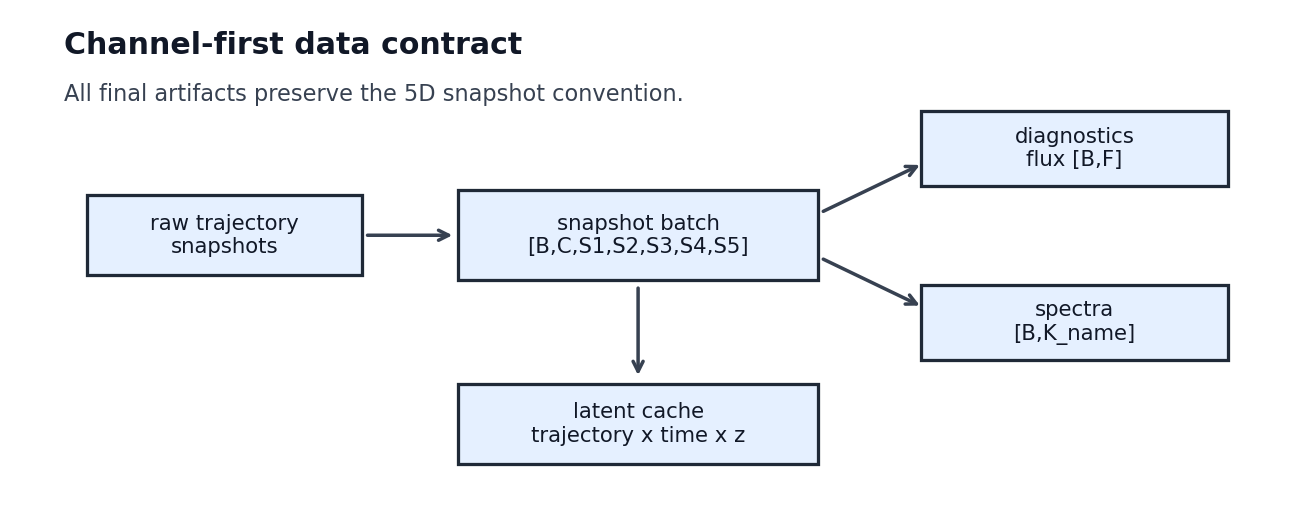
\includegraphics[width=0.95\textwidth]{data_contract_diagram.png}
  \caption{Data and latent-cache contracts. Splits are defined at trajectory level so overlapping
  windows from one trajectory cannot appear in both training and evaluation.}
  \label{fig:data-contract}
\end{figure}

Trajectories are deterministically shuffled using a fixed seed and assigned with ratios
$0.8/0.1/0.1$. For the medium cache this produces 41 training, five validation, and five test
trajectories. Each trajectory contains 23 retained time steps, giving 1,173 latent vectors. Splitting
before window construction is essential: randomly splitting overlapping windows would leak nearly
identical temporal contexts across partitions.

For context length $T_c$ and prediction length $T_p$, a valid window begins at any index
$i\in\{0,\ldots,T-T_c-T_p\}$. The principal sequence experiment uses $T_c=8$ for one-step training
and recursive evaluation over $T_r=8$ forecast steps.

\section{Snapshot Encoder}

The selected encoder is a five-dimensional pointwise convolutional hierarchy. The input channel
axis is moved to the end for Flax operations. Each of three stages first subsamples the five spatial
axes and then applies a learned pointwise projection with 8, 16, and 32 output channels. The stride
vectors are
\begin{align}
  (2,2,2,4,2),\quad (2,1,2,4,2),\quad (2,1,1,2,2).
\end{align}
GELU activations follow each projection. Global mean pooling over all remaining spatial positions
produces one vector, and a dense layer maps it to $z_t\in\mathbb{R}^{128}$.

The $1^5$ kernels make this architecture computationally tractable for the large input tensor. Its
spatial mixing comes primarily from subsampling and global pooling rather than wide convolutional
kernels. This is an engineering baseline, not a claim that pointwise operations optimally represent
gyrokinetic geometry.

\section{Representation Objective}

Two augmented views are sampled independently from a snapshot. The enabled transforms are Gaussian
noise with relative scale $0.01$, amplitude jitter of $0.02$, and element masking with probability
$0.02$. Let $g$ be a two-layer projection head and $h$ a prediction head. The symmetric SimSiam loss
is
\begin{equation}
  \mathcal{L}_{\mathrm{Siam}}
  =\frac{1}{2}\left[-\cos\left(h(g(f(x^{(1)}))),\operatorname{sg}(g(f(x^{(2)})))\right)
  -\cos\left(h(g(f(x^{(2)}))),\operatorname{sg}(g(f(x^{(1)})))\right)\right],
\end{equation}
where $\operatorname{sg}$ denotes stop-gradient.

The latent vector is also passed to independent diagnostic heads. Each head contains a 256-unit
hidden layer and predicts scalar flux or a 32-bin spectrum. With mean squared diagnostic losses,
the encoder objective is
\begin{equation}
  \mathcal{L}_{\mathrm{enc}}
  = \mathcal{L}_{\mathrm{flux}}
  + \mathcal{L}_{\mathrm{spectra}}
  + 0.5\,\mathcal{L}_{\mathrm{Siam}}.
\end{equation}
Both spectra, \code{kyspec} and \code{fluxspec}, are used in the spectra term. The diagnostic heads
make the representation task-aware, while the Siamese term encourages consistency under the small
perturbations shown in \autoref{fig:encoder-objective}.

\begin{figure}[htbp]
  \centering
  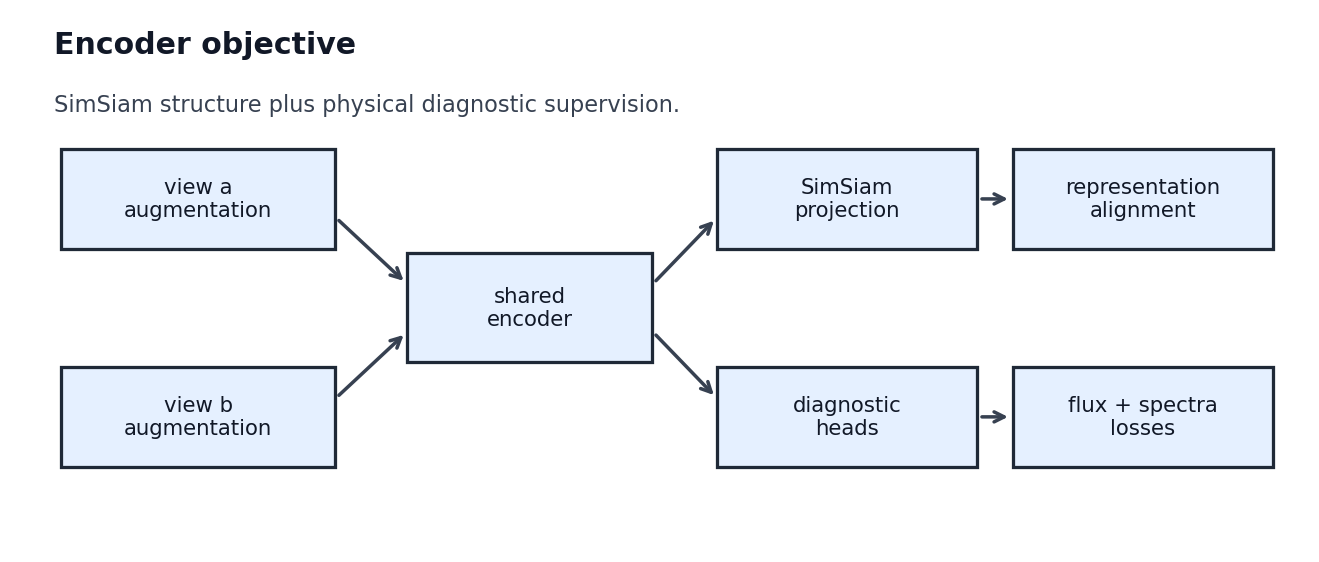
\includegraphics[width=0.92\textwidth]{encoder_objective_diagram.png}
  \caption{Joint encoder training objective: two conservative augmented views are aligned with a
  stop-gradient Siamese objective, while flux and spectra heads retain diagnostic information.}
  \label{fig:encoder-objective}
\end{figure}

\section{Latent Cache}

After encoder training, every trajectory is embedded once. The HDF5 cache stores $z_t$, timestep
indices, physical time when available, flux, spectra, the encoder checkpoint path, and the resolved
configuration. This immutable boundary has two benefits: temporal models can be iterated without
re-reading five-dimensional fields, and all compared sequence models receive identical inputs.

For cache normalization, the mean $\mu_z$ and standard deviation $\sigma_z$ are computed from the
training trajectories only. Sequence learning then uses
\begin{equation}
  \tilde z_t = \frac{z_t-\mu_z}{\sigma_z+\epsilon},\qquad \epsilon=10^{-6}.
\end{equation}
Predictions are transformed back before the frozen diagnostic heads are evaluated. Restricting the
statistics to the training split prevents test information from entering preprocessing.

\section{Sequence Models}

\subsection{Persistence}

The persistence baseline predicts
\begin{equation}
  \hat z_{t+1}=z_t
\end{equation}
and repeats this value during recursive rollout. It is difficult to beat when adjacent states change
slowly, making it a necessary baseline for short-horizon dynamics.

\subsection{GRU}

The recurrent baseline uses one GRU layer with hidden width 256 and a dense output projection to
128 dimensions. It consumes the eight context latents sequentially and predicts the next latent
from the final hidden state.

\subsection{Causal Transformer}

The selected Transformer projects each 128-dimensional latent to width 256, adds learned positional
embeddings, and applies three pre-normalized causal self-attention blocks. Each block has four
attention heads and an MLP expansion ratio of four. The normalized final context token is projected
back to 128 dimensions. Dropout is zero in the medium experiment.

All learned sequence models minimize a latent objective combining mean squared error and cosine
dissimilarity. Adam-style optimization uses learning rate $10^{-3}$, weight decay $10^{-4}$, a
25-step warmup, and gradient-norm clipping at one. Models are trained for 500 update steps.

\section{Autoregressive Evaluation}

Given true context $z_{t-T_c+1:t}$, the model predicts $\hat z_{t+1}$. The context window is shifted,
the prediction is appended, and the procedure is repeated for eight steps. The persistence baseline
uses the same window construction. For latent prediction $\hat Z$ and target $Z$, the principal
latent metric is
\begin{equation}
  \mathrm{MSE}_{z}=\frac{1}{BT_rD}\lVert \hat Z-Z\rVert_2^2.
\end{equation}

Flux RMSE is computed after applying the frozen flux head $d_f$:
\begin{equation}
  \mathrm{RMSE}_{f}=\sqrt{\frac{1}{BT_r}\sum_{b=1}^{B}\sum_{k=1}^{T_r}
  \left(d_f(\hat z_{b,k})-f_{b,k}\right)^2}.
\end{equation}
Spectra MSE, log-MSE, relative $L_2$, and shape correlation are reported as secondary diagnostics.
A rollout is stable when every predicted value is finite.

Overlapping windows can cause long trajectories to dominate a sample-weighted aggregate. The
verified evaluation first computes metrics per trajectory and then gives each test trajectory equal
weight. Dispersion therefore represents between-trajectory variation. Horizons are one-based in
reports, so horizon one denotes the first predicted state.

\cleardoubleoddpage
\chapter{Implementation}
\label{chap:implementation}

\section{Software Architecture}

The implementation is organized as a Python package named \code{gk\_surrogate}. Configuration,
data access, models, training, evaluation, metrics, and device-parallel utilities are separate
modules. The public command-line interface exposes six principal operations:

\begin{enumerate}
  \item inspect a dataset and validate its shape and targets;
  \item train an encoder;
  \item embed trajectories into a latent cache;
  \item evaluate a frozen flux head and plot the representation;
  \item train a latent sequence model; and
  \item evaluate an autoregressive rollout.
\end{enumerate}

YAML experiment files are validated with Pydantic schemas and written back as resolved
configuration artifacts. Environment variables supply machine-specific paths. This makes the
scientific protocol reviewable without hard-coding the server layout in source code.

\section{Data Adapters}

All raw data sources implement the same trajectory interface: enumerate trajectory identifiers,
report the number of time steps and snapshot shape, and retrieve a snapshot plus diagnostics. A
synthetic generator supports deterministic end-to-end tests. A generic HDF5 adapter supports small
fixtures and alternative schemas. The principal real-data adapter reads the confirmed
Cyclone/KvikIO directory layout and maps upstream fields into the internal channel-first contract.

The direct reader detects float32 and BF16 shard availability, but arrays presented to model code
are float32. The selected data configuration uses the distribution field \code{df}, offset 80,
temporal subsampling by eight, spatial inverse transforms, and stored 32-bin \code{kyspec} and
\code{fluxspec} targets. Potential-field input is supported by generic adapters but is not part of
the selected evidence.

File operations are deliberately outside \code{jax.jit}. NumPy and HDF5 objects are converted at
the boundary, after which training steps accept JAX arrays. This prevents Python I/O from being
captured by compiled computations.

\section{JAX Execution and Parallelism}

Model computations use Flax Linen modules. Training steps are pure enough to be transformed with
automatic differentiation and just-in-time compilation. Optax composes warmup, Adam-style updates,
weight decay, and gradient clipping. Random keys are explicit and derived from fixed experiment
seeds.

The same source supports single-device execution and single-host data parallelism. In automatic
mode, batches are sharded across visible devices and the code uses \code{pmap}; no GPU count is
hard-coded. The medium experiments recorded four CUDA devices. Portable tests set
\code{JAX\_PLATFORM\_NAME=cpu} and use tiny synthetic tensors. Multi-node execution is outside the
scope of the thesis.

\section{Verification Strategy}

Verification is layered. Unit tests cover shape guards, configuration consistency, data adapters,
normalization, splits, augmentations, losses, model forward passes, training steps, metrics,
checkpointing, and CLI contracts. A synthetic smoke pipeline executes the complete lifecycle from
inspection to rollout plots without real data or a GPU. Static checks include Ruff and mypy, and the
test gate enforces at least 95\% line coverage. Packaging is checked by building both a source
distribution and wheel.

The synthetic pipeline is engineering evidence, not a scientific result. Its purpose is to detect
interface regressions and verify that the repository remains executable independently of private
data and hardware.

\section{Provenance and Artifact Policy}

Each experiment output records its resolved config, Git state, metrics, and device report when
applicable. Checkpoints and latent caches store metadata linking them to upstream artifacts. Raw
data, checkpoints, HDF5 caches, generated plots, W\&B state, and build products are excluded from
version control. Thesis-facing documentation records stable tables and claim boundaries while
large artifacts remain in ignored storage.

This policy also separates protocol tiers. Synthetic smoke runs establish software correctness;
one-trajectory and small experiments establish data binding and validation behavior; the medium
cache supplies the main quantitative comparison. Numbers from different caches, splits, horizons,
or aggregation rules are not combined in one headline table.

\cleardoubleoddpage
\chapter{Experimental Setup}
\label{chap:experiments}

\section{Evidence Tiers and Frozen Scope}

The repository separates engineering evidence from thesis evidence. Synthetic smoke runs test
that the data contract, encoder, cache, sequence trainer, rollout evaluator, and report writers
execute without private data or a GPU. Small real-data checks validate the Cyclone/KvikIO schema
and target fields. Only the byte-verified medium universe and its frozen protocol enter the
scientific comparison. This separation is important: a successful command is not evidence that a
surrogate generalizes.

The accepted comparison is a retrospective five-fold nested group cross-validation study. The
51-trajectory universe was available for development and its manifest is therefore not a pristine
locked test set. Each outer fold holds out trajectories that are disjoint from its training and
inner-validation groups. Model and checkpoint choices are made inside the fold, before the outer
test evidence for that fold is opened. The reported uncertainty is an estimate of performance on
this finite universe, not a claim of deployment-level generalization.

\section{Medium Dataset and Data Binding}

The consumed universe contains 51 trajectories and 1,173 retained timestep bundles. Every
trajectory contributes 23 retained time steps under the preprocessing contract: four input
channels, spatial shape $(32,8,16,85,32)$, offset 80, temporal subsampling by eight, stored
$\code{kyspec}$ and $\code{fluxspec}$ targets, and a preferred float32 representation. The
channel-first snapshot contract is
\begin{equation}
  x \in \mathbb{R}^{B\times C\times S_1\times S_2\times S_3\times S_4\times S_5}.
\end{equation}
The byte-level universe manifest records the ordered trajectory identifiers, the 1,173 sampled
binary timestep files, and the metadata files required by the loader. Both the durable consumed
subset and the operational public-data alias were checked against the same manifest by hashing
each consumed file; no path is used as a dataset identity.

The five outer folds contain 30 or 31 training trajectories, 10 or 11 validation trajectories,
and 10 or 11 test trajectories. The exact fold manifests are committed under
\path{experiment_protocols/} and are addressed by their SHA-256 digest. Within each fold, all
normalization statistics, encoder parameters, latent caches, and sequence checkpoints are derived
from the fold's training trajectories. This is an end-to-end split: a trajectory used by an
encoder is never called an outer-test trajectory for that fold.

\section{Representation and Temporal Models}

The convolutional encoder maps each preprocessed snapshot to a 128-dimensional latent state. Its
training objective combines a SimSiam-style consistency term with supervised heads for scalar flux
and the two one-dimensional spectra. The heads are retained after encoder training so that a
latent rollout can be evaluated in the original diagnostic space. The work deliberately does not
claim five-dimensional field reconstruction; the decoder required for that claim is outside the
scope of the study.

The sequence candidates are a gated recurrent unit (GRU) and a causal Transformer. Latent-state
persistence is the primary latent-dynamics reference, and direct persistence of the observed flux
is the primary diagnostic baseline. An additional diagnostic-head oracle applies the frozen head
to true future latents. It is an analysis control: it is not a forecast and cannot be interpreted
as an achievable model result. All learned candidates use the same eight-step context, recursive
eight-step forecast horizon, diagnostic lineage, and trajectory-balanced metrics.

Each sequence trainer runs for 500 updates. The GRU has one 256-unit layer; the Transformer uses
width 256, depth three, four attention heads, and no dropout. The cache-normalized variants fit
latent normalization on training trajectories only. Sequence checkpoints are selected by the
lowest validation trajectory-balanced latent RMSE. This checkpoint rule is distinct from family
selection: after each candidate has a validation checkpoint, the GRU or Transformer family with
the lower arithmetic mean of validation trajectory-balanced flux RMSE across seeds is selected
within that outer fold.

\section{Matched Seeds and Stage Ledger}

The development/data seed is fixed at 52. Training seeds are matched across learned candidates at
52, 53, 54, 55, and 56, so initialization variability is visible without changing the trajectory
universe. Persistence controls are evaluated on the same trajectories and horizons and do not
  receive a fictitious training seed. The frozen stage plan contains 255 slots: 230 accepted
  ledger slots (225 metric stages and five selection barriers) and 25 explicitly skipped
  unselected-family test stages. No stage is silently
dropped, retried into the accepted set, or selected from an outer-test metric.

The outer-fold family selections are Transformer for folds 0, 1, and 3, and GRU for folds 2 and
4. This is a fold-wise selection result, not evidence that one architecture is a global winner.
The release manifest records all 25 fold--seed rows, the selected family, stage configuration
hashes, and the exact accepted/skipped counts without publishing trajectory identifiers or server
paths.

\section{Metrics and Estimands}

Flux RMSE is the primary metric because the research question concerns diagnostic forecasting. It
is computed per trajectory and then averaged, so a trajectory with many overlapping windows cannot
dominate a trajectory with fewer valid windows. Latent MSE, flux MAE, spectral relative $L_2$ error,
spectral shape correlation, and finite-output stability are secondary diagnostics. Values are in
preprocessed target units; no physical-unit conversion is claimed.

The primary estimand is the selected learned model minus observed-flux persistence difference in
per-trajectory flux RMSE, averaged hierarchically with equal outer-fold, training-seed, and
trajectory weights. A paired hierarchical bootstrap \citep{saravanan2020hierarchical} resamples training seeds and trajectories
within the fold structure; its 10,000 replicates use a fixed seed recorded in the aggregate. The
secondary estimand is the analogous learned-minus-latent-persistence difference in latent MSE.
We report both point estimates and intervals, plus per-seed variability and a hierarchically
weighted fraction of improved trajectory runs. If the primary interval includes zero, the protocol
requires the conclusion ``no convincing advantage''; a negative result is valid evidence, not a
reason to change the selection rule.

Spectra are reported separately for $\code{kyspec}$ and $\code{fluxspec}$, with relative error and
shape correlation shown together. Their scales and norms differ, so a single pooled spectral
number is not used to claim physical fidelity. No transfer-learning, full-field reconstruction,
long-horizon, solver-speed, or GyroSwin comparison is part of the evidence set.

\section{Reproducibility and W\&B Policy}

The protocol, fold manifests, resolved configuration hashes, stage evidence, and release manifest
form a chain from source tag to result. Raw data, checkpoints, latent caches, and per-trajectory
rows remain outside Git. W\&B is disabled for all 225 accepted metric stages; local status files explicitly
record \code{enabled=false}, \code{requested=false}, and \code{mode=disabled}. Consequently the
thesis cites no live W\&B run or URL. The local manifest, not an online dashboard, is the source of
truth for this result.

\cleardoubleoddpage
\chapter{Results}
\label{chap:results}

\section{Evidence and Selection Integrity}

The accepted release is generated from the frozen protocol tag
\texttt{protocol/multiseed-v1} (source commit prefix \texttt{be976808}; the full digest is in
Appendix~\ref{app:reproducibility}). The
dataset revision is the byte-verified consumed universe with revision digest
\texttt{cyclone-consumed-bytes-sha256:ff2867e9}; the universe and outer-fold manifest digests are
\texttt{96c85a70} and \texttt{da5d95b8}, respectively (the complete values are in the release
manifest). The evidence tree contains 255 planned stage slots: 230 accepted ledger slots (225
metric stages and five selection barriers) and 25 skipped because
their learned family was not selected. There are no invalidated accepted rows.

Every accepted metric stage is finite and stable, uses the declared fold and training seed, and records
the expected checkpoint/cache lineage. The five selection records all report
\code{test\_evidence\_opened=false}. The W\&B contract is disabled and verified for every accepted metric stage.
These checks matter because a numerically plausible rollout can still be scientifically invalid if
an encoder has seen its supposed test trajectories or if an unselected test model was inspected.

\section{Qualitative Latent-Space Geometry}

\autoref{fig:latent-space} visualizes all 1,173 encoded snapshots from one reconstructed
protocol run: outer fold 0, training seed 52. The trajectory roles come directly from the frozen
fold manifest, rather than from a second random split. Colour represents the preprocessed scalar
flux target; marker shape identifies the training, validation, or test role. PCA gives a linear
view, while t-SNE at perplexities 5 and 30 gives two local-neighbourhood views under the same seed.

\begin{figure}[htbp]
  \centering
  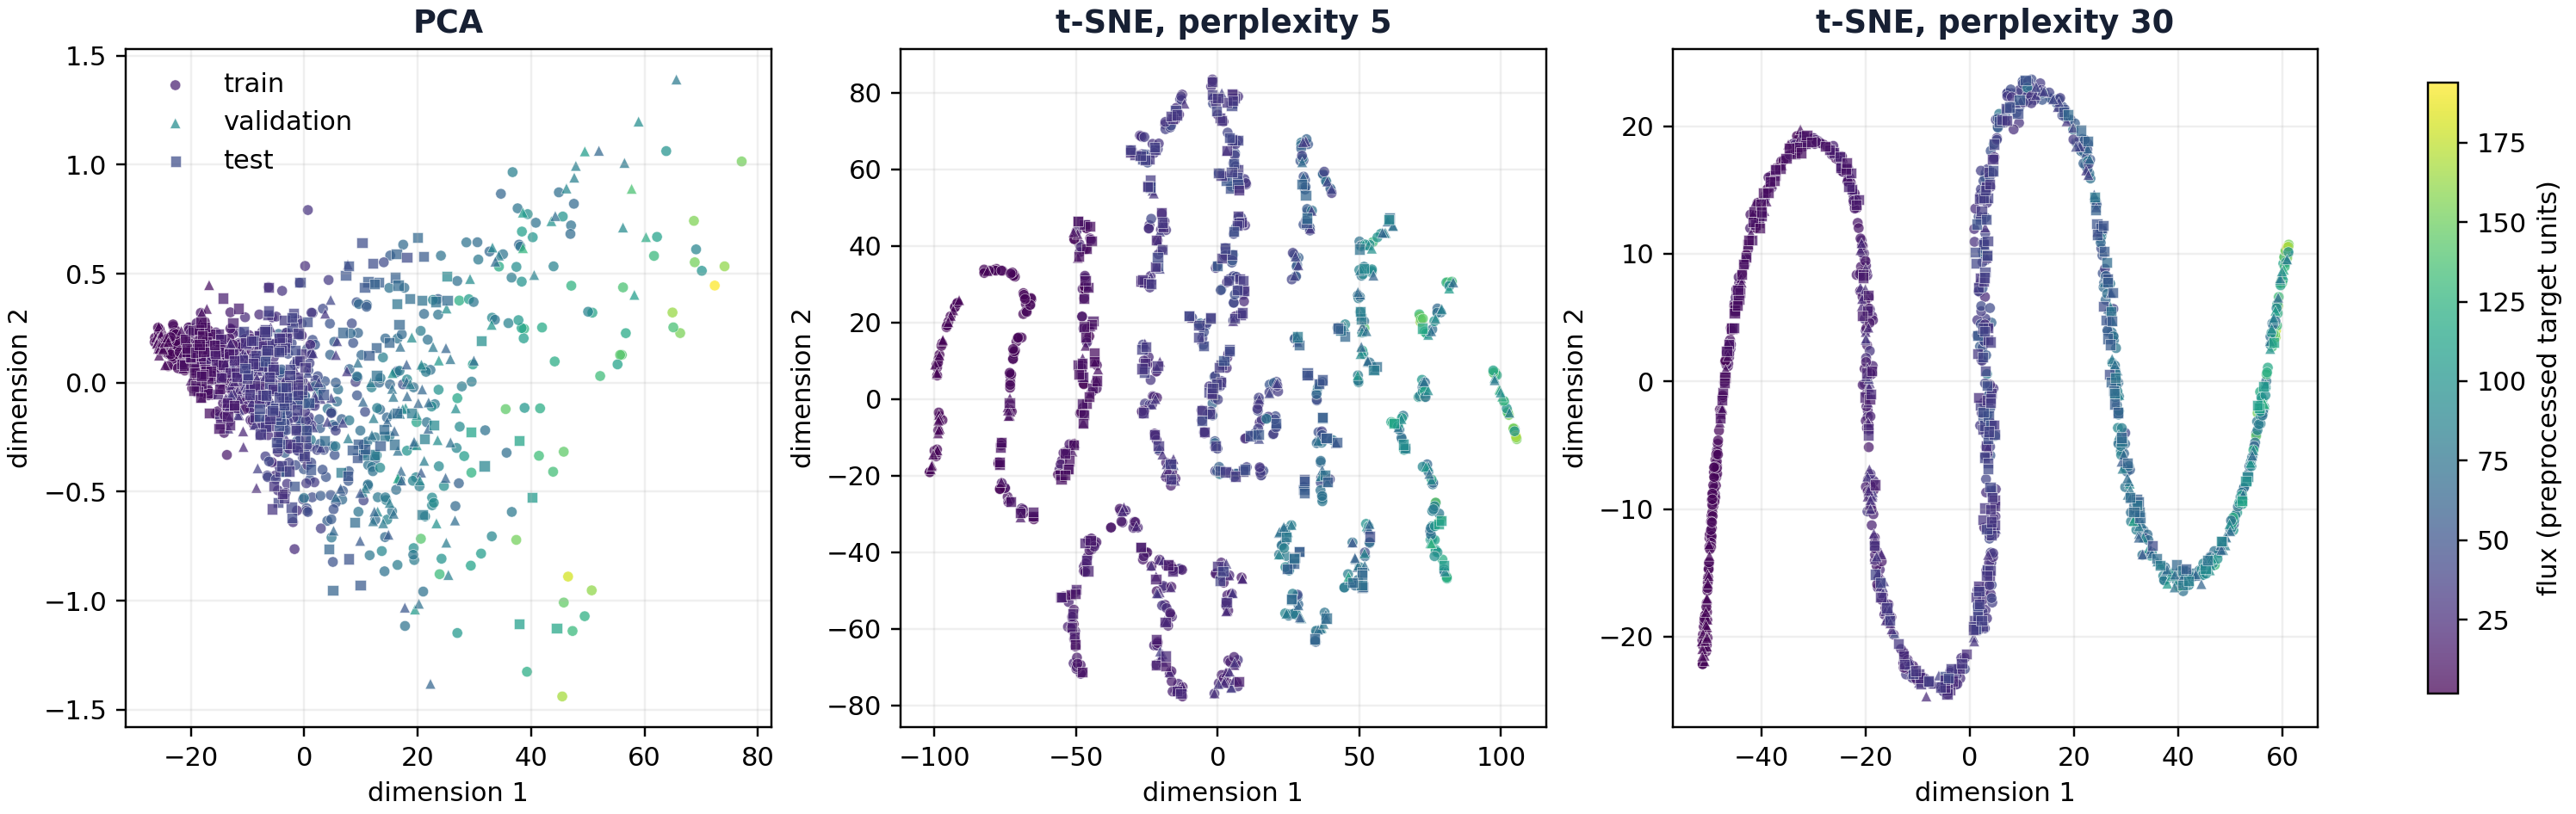
\includegraphics[width=\textwidth]{latent_space_projection.png}
  \caption{Qualitative latent-space geometry for all 1,173 points in the canonical
  \texttt{multiseed-v1} outer-fold-0, seed-52 cache. Colour denotes preprocessed flux and marker
  shape denotes the exact manifest role. This is one protocol-bound run, not an aggregate
  multiseed performance estimate. The t-SNE axes and global distances have no physical meaning,
  and the panels do not establish split separation or model superiority.}
  \label{fig:latent-space}
\end{figure}

The projections are descriptive only. There is no shared latent coordinate system across the 25
fold--seed encoder fits, so averaging their coordinates would not define a meaningful multiseed
plot. The visible flux ordering is compatible with the supervised diagnostic objective, but it is
not a held-out accuracy result and does not imply that the representation retains the full
five-dimensional state.

\section{Outer-Fold Selection}

The fold-level family choices are shown in \autoref{tab:fold-selection}. The selection means are
computed from five matched validation seeds; the table does not use outer-test metrics. The
variation in selected family is itself a result: the evidence does not justify naming a single
globally superior architecture.

\begin{table}[htbp]
  \centering
  \caption{Architecture selected independently in each outer fold. Selection uses the mean
  validation trajectory-balanced flux RMSE over seeds 52--56; lower is better.}
  \label{tab:fold-selection}
  \small
  \begin{tabular}{lrrr}
    \toprule
    Outer fold & Test trajectories & Selected family & Validation selection rule \\
    \midrule
    0 & 11 & Transformer & five-seed mean flux RMSE \\
    1 & 10 & Transformer & five-seed mean flux RMSE \\
    2 & 10 & GRU & five-seed mean flux RMSE \\
    3 & 10 & Transformer & five-seed mean flux RMSE \\
    4 & 10 & GRU & five-seed mean flux RMSE \\
    \bottomrule
  \end{tabular}
\end{table}

The selection is deliberately two-level. Within each seed, a sequence checkpoint is chosen by
validation latent RMSE. The family comparison then averages the resulting validation flux RMSE
over all five training seeds. This distinction prevents the flux metric from silently becoming a
test-aware checkpoint rule and prevents a single lucky initialization from determining the family.

\section{Primary Diagnostic Result}

The primary estimand is the selected learned model minus direct observed-flux persistence in
trajectory-balanced flux RMSE. The aggregate learned error is 14.6729, whereas observed
persistence is 10.0207. The difference is therefore +4.6522 in favour of the baseline. The paired
hierarchical bootstrap interval is [+2.5788, +6.6470], based on 10,000 replicates and the frozen
bootstrap seed. It is entirely above zero, so the protocol's negative-result rule applies: the
learned surrogate shows no convincing advantage and is, on this metric and universe, worse than
the simple observed diagnostic persistence.

\begin{table}[htbp]
  \centering
  \caption{Primary outer-test estimate across five folds and five matched seeds. Positive
  differences mean that the learned model has larger error than observed persistence.}
  \label{tab:primary-results}
  \small
  \begin{tabularx}{\textwidth}{>{\raggedright\arraybackslash}X r >{\raggedright\arraybackslash}X}
    \toprule
    Quantity & Value & Interpretation \\
    \midrule
    Selected learned flux RMSE & 14.6729 & lower is better \\
    Observed-flux persistence flux RMSE & 10.0207 & primary baseline \\
    Learned minus observed difference & +4.6522 & baseline advantage \\
    Hierarchical bootstrap 95\% interval & [+2.5788, +6.6470] & excludes zero \\
    Hierarchically weighted improved fraction & 31.6\% & learned error lower \\
    Paired fold--seed--trajectory rows & 255 & finite and paired \\
    \bottomrule
  \end{tabularx}
\end{table}

The hierarchically weighted fraction is not a claim that exactly 31.6\% of raw rows are an
independent sample; it gives equal weight to folds and seeds before trajectory averaging. The
per-fold point differences are positive in all five folds: +1.4189, +3.9495, +6.5372, +7.2051,
and +4.1503. Thus the negative conclusion is not caused by one pathological outer split, although
the magnitude varies substantially between folds.

\begin{figure}[htbp]
  \centering
  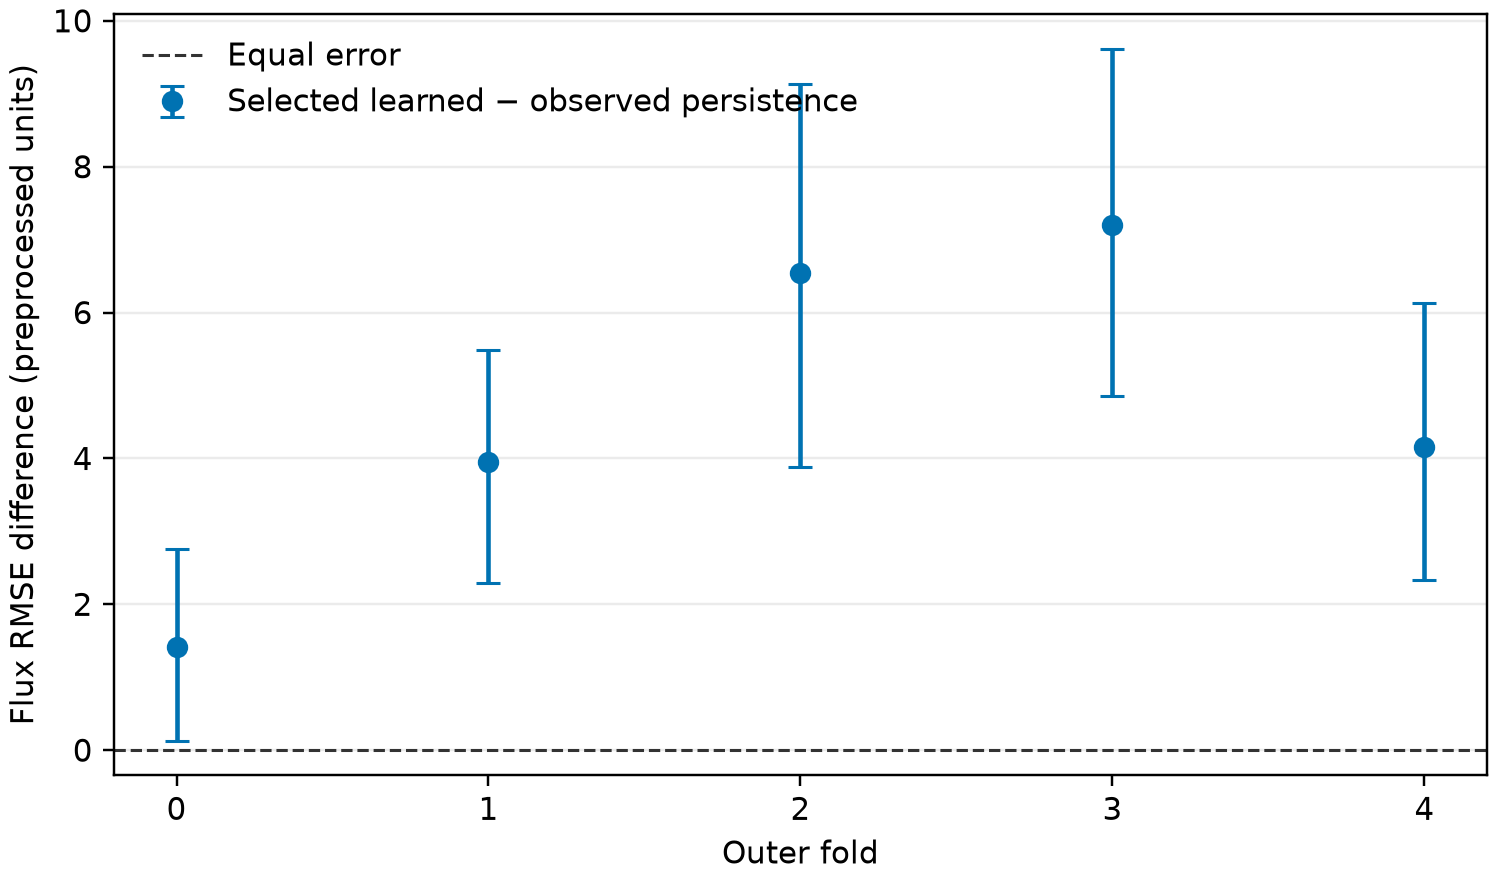
\includegraphics[width=0.78\textwidth]{verified_primary_by_fold.png}
  \caption{Selected-model minus observed-persistence flux RMSE by outer fold. Points are fold
  means and bars are the release's fold-level bootstrap intervals. The zero line marks equal
  performance; every fold is on the positive-error side.}
  \label{fig:primary-by-fold}
\end{figure}

\section{Latent Dynamics and Forecast Horizon}

Decoded latent-state persistence has flux RMSE 14.8049, only slightly worse than the selected
learned models at the aggregate level. This is a useful reference because it asks whether a
sequence model improves on holding the encoded state fixed, but it is not the primary diagnostic
baseline: it still passes through the learned diagnostic head. The diagnostic-head oracle, which
receives the true future latents, reaches flux RMSE 12.3732. It is better than either latent
rollout but remains worse than observed persistence. The result therefore identifies a material
representation-to-diagnostic gap without isolating a single cause; the oracle is a control, not a
forecast ceiling.

The secondary latent estimand is selected learned minus latent-persistence latent MSE. Learned
latent MSE is 0.4497 versus 0.4307 for persistence, giving +0.0189. Its interval
[-0.0699, +0.1332] includes zero. Accordingly, the experiment does not support a claim that the
sequence model improves latent dynamics either. The point estimate is compatible with a small
regression or improvement under another realization, and the interval is the correct summary of
that uncertainty.

\begin{figure}[htbp]
  \centering
  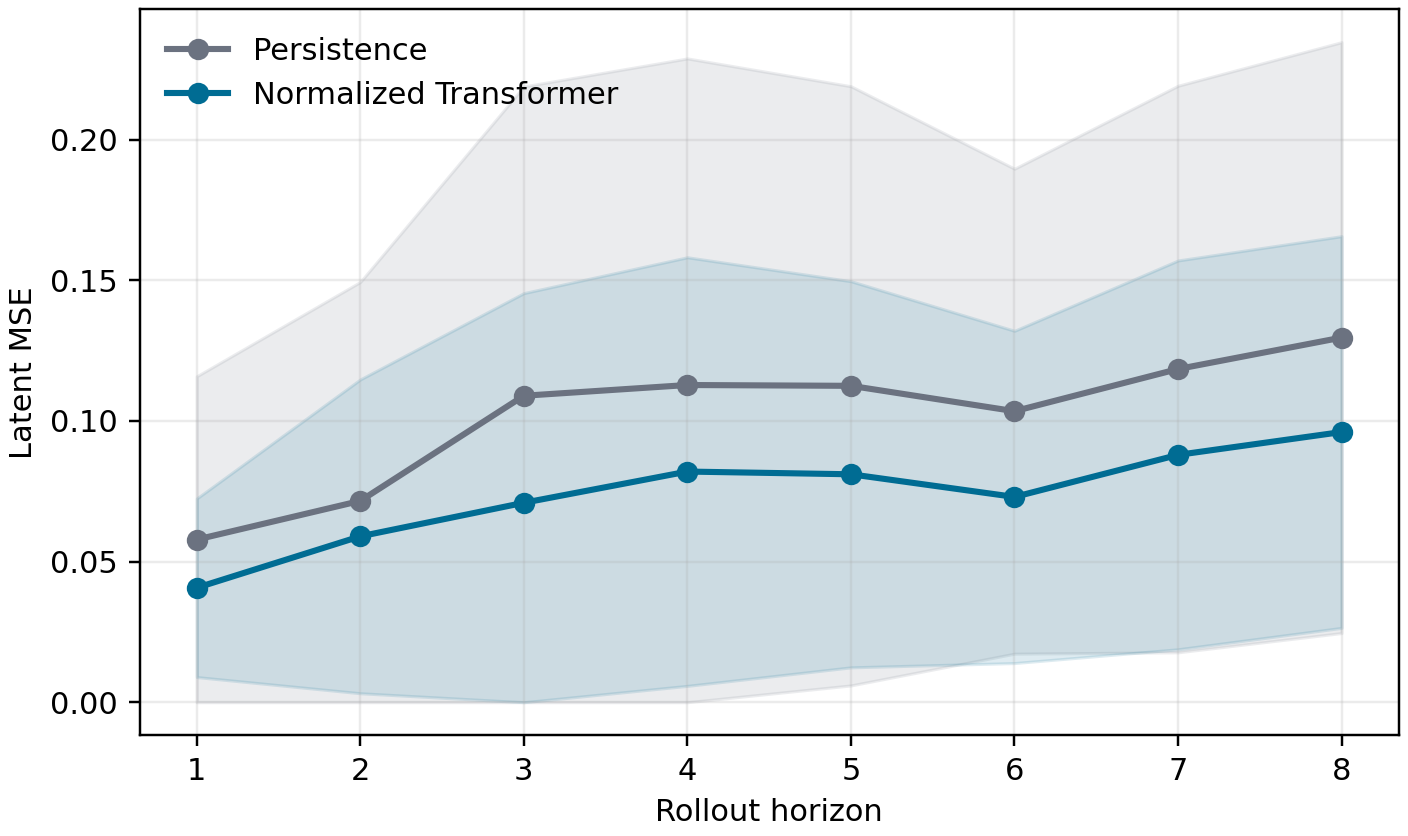
\includegraphics[width=0.78\textwidth]{verified_latent_mse_by_step.png}
  \caption{Mean latent MSE by forecast step across outer folds. The ribbon is the standard
  deviation between outer-fold means; it is not a confidence interval. Curves are generated from
  the release's fold-level by-step arrays rather than from a selected seed.}
  \label{fig:latent-horizon}
\end{figure}

\begin{figure}[htbp]
  \centering
  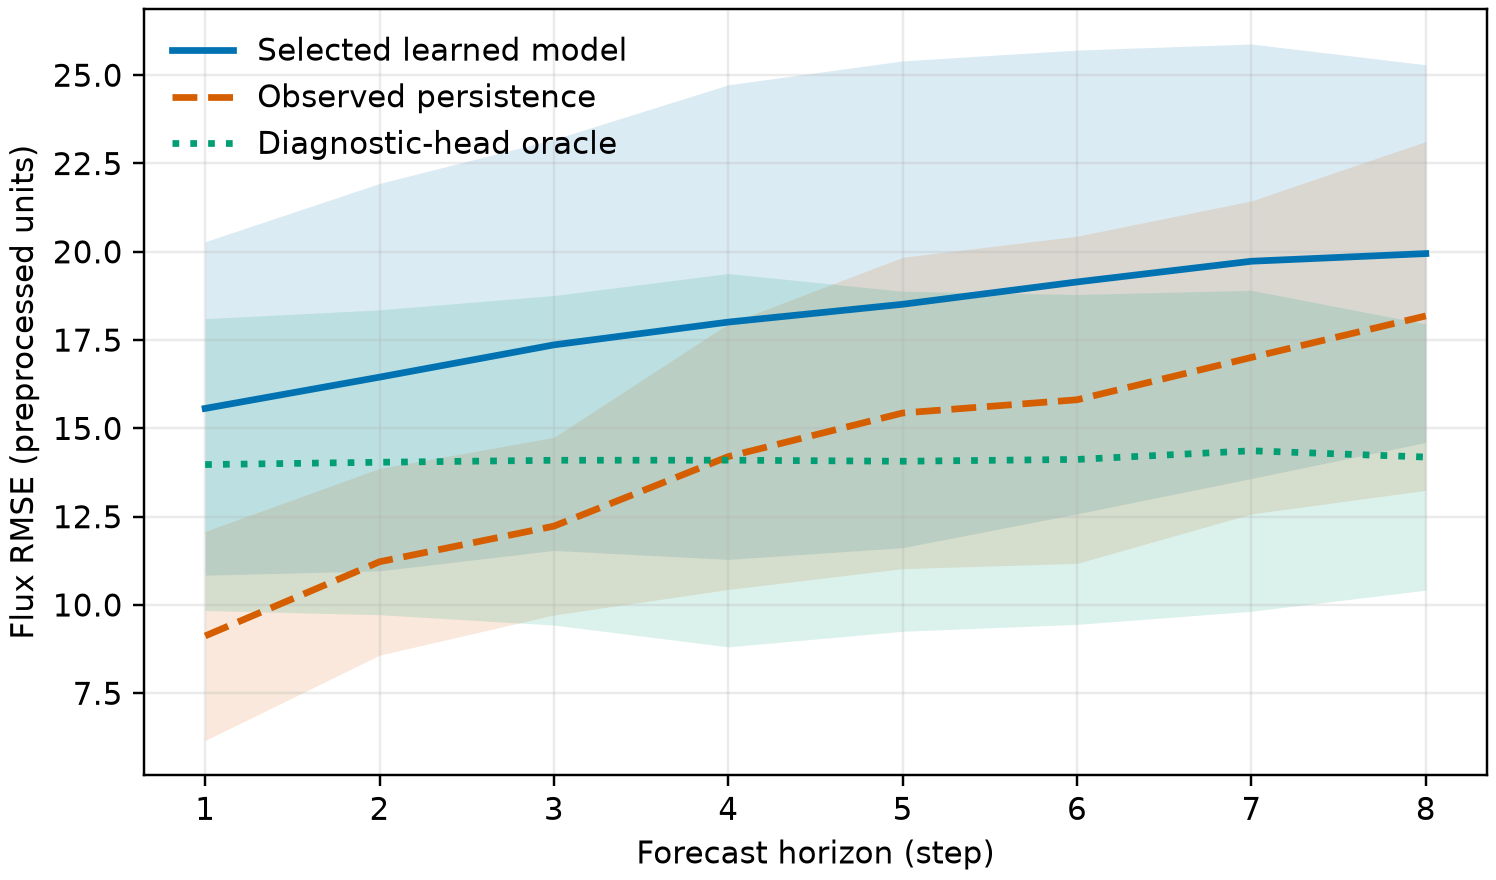
\includegraphics[width=0.78\textwidth]{verified_flux_rmse_by_step.png}
  \caption{Mean diagnostic flux RMSE by forecast step for the selected learned model, observed
  persistence, and the diagnostic-head oracle. Shaded ribbons show between-outer-fold standard
  deviation, not confidence intervals. The figure is a horizon diagnostic, not a new selection
  criterion.}
  \label{fig:flux-horizon}
\end{figure}

The horizon curves remain finite, but finiteness is a stability check rather than an accuracy
claim. In particular, a rollout can be numerically stable while drifting systematically away from
the observed diagnostic. The positive aggregate difference and the per-fold results are therefore
more important than the absence of exploding values.

\section{Spectral Diagnostics}

Spectral results are kept per target, as required by the protocol. For $\code{fluxspec}$, the
learned relative $L_2$ error is 1.5026 with shape correlation 0.6011, compared with 0.4433 and
0.9123 for observed persistence. For $\code{kyspec}$, the learned relative $L_2$ error is 28.1003
with shape correlation 0.7226, compared with 0.5296 and 0.9330 for observed persistence. Decoded
latent persistence is similarly worse than observed persistence (relative $L_2$ 1.4597 for
\code{fluxspec} and 27.2029 for \code{kyspec}).

These large, target-dependent relative errors are not combined into a single claim of spectral
fidelity. The shape correlations show that some broad spectral ordering is retained, while the
scale-sensitive errors show that this is insufficient for quantitative prediction. Spectra
therefore reinforce, rather than overturn, the primary flux result.

\section{Answer to the Research Questions}

RQ1 asks whether the compact state retains diagnostic information. The finite oracle and nontrivial
spectral correlations show that the representation carries usable signal, but the oracle's error
relative to observed persistence shows that it is not sufficient for accurate diagnostic rollout.
RQ2 asks whether a learned sequence model beats observed persistence. Across the frozen nested
cross-validation estimate, it does not: the interval for learned minus observed flux RMSE is
strictly positive. RQ3 asks whether the cache-normalized architecture is a reliable winner. The
fold selections alternate between GRU and Transformer, so no global winner is supported.

No historical seed-52 values, mixed-split runs, unpaired exploratory baselines, or external
architecture numbers are used in these conclusions. The negative result is bounded to the
51-trajectory universe, the preprocessing contract, the eight-step horizon, and the declared
diagnostic targets.

\cleardoubleoddpage
\chapter{Discussion}
\label{chap:discussion}

\section{Answer to the Research Question}

The cache-normalized Transformer is the best learned model on validation flux RMSE. In the
retrospective seed-52 test realization, its flux RMSE is 11.4255, compared with 11.9889 for
decoded latent persistence and 3.7208 for direct persistence of the observed flux. Applying the
frozen diagnostic head to true future latents gives 12.0712, so the learned model does not beat the
appropriate observed-diagnostic baseline and the comparison does not establish superiority.

The run establishes that the complete data, representation, cache, sequence, diagnostic, and
provenance path can be executed with a strict trajectory-level split. It also shows that the
observed diagnostic is a much stronger reference than decoded latent persistence, and that a
complex temporal architecture does not by itself demonstrate useful forecasting. The oracle
result identifies diagnostic decoding as a limiting factor under the present encoder and budget.

\section{Interpretation of the Test Difference}

The Transformer and observed-persistence flux RMSE values differ by 7.7047 in the trajectory-balanced
headline, with the learned error 3.07 times as large. The five trajectory-level differences
(Transformer minus observed persistence) have mean 7.7902 and a descriptive 95\% interval from
$-0.6813$ to $16.2616$. The current design has only one sequence-training seed and five
trajectories, so this interval is descriptive and does not establish repeatability.

The Transformer has lower latent error than decoded latent persistence, but that comparison shares
the diagnostic head and is secondary to the observed-diagnostic baseline. The modest spectral
differences occur without a meaningful change in aggregate shape correlation. These disagreements
justify the metric hierarchy: observed-flux RMSE is primary, while latent error, MAE, and spectra
diagnostics explain the failure mode.

The learned model also has lower latent MSE than decoded latent persistence on the retrospective
test. Because diagnostic heads are nonlinear and task-specific, latent and observed-diagnostic
rankings need not match. Cache normalization improved both learned architectures on validation,
but matched multi-seed runs are needed before treating that effect as repeatable.

\section{Importance of the Integrity Audit}

The most consequential finding was methodological rather than architectural. Different trajectory
split seeds had previously been used for encoder training and downstream evaluation. A trajectory
can then be called ``test'' downstream even though its snapshots were used to train the encoder,
which violates end-to-end held-out evaluation. The resulting metric may still measure sequence-model
behaviour on a fixed cache, but it cannot support a claim about generalization of the complete
surrogate.

Withdrawing the earlier result is necessary scientific hygiene. The corrected system now binds
every cache and checkpoint to its split seed, records exact trajectory manifests, fits normalization
statistics on training trajectories only, and rejects incompatible artifacts before evaluation.
These controls are more valuable than retaining a numerically stronger but invalid headline. They
also make future negative or positive results easier to audit.

\section{Comparison with Related Work}

GyroSwin predicts full five-dimensional dynamics and targets physically motivated field validation
at a larger architectural scale \citep{paischer2025gyroswin}. The present system instead evaluates a
128-dimensional diagnostic-oriented state without a decoder. The two approaches therefore answer
different questions: field fidelity versus compact diagnostic prediction.

A direct accuracy comparison remains invalid without the same data revision, trajectory split,
temporal sampling, target definitions, normalization, forecast horizon, and aggregation. The
internal result does not imply that latent surrogates in general are superior to full-field
models, nor does it provide evidence about GyroSwin performance. It only constrains the specific
encoder, learned sequence candidates, data subset, and budget evaluated here.

\section{Limitations}

The study has several limitations:

\begin{itemize}
  \item The medium cache contains 51 trajectories from one preprocessing pipeline. Five validation
        and five test trajectories provide limited independent coverage of the underlying regime.
  \item Each learned candidate is trained once, and the GRU and Transformer use different fixed
        training seeds. Multiple matched seeds are required to separate architecture from
        initialization variability and assess repeatability.
  \item The eight-step horizon establishes short-term behaviour only. It does not demonstrate
        long-term stability or error saturation.
  \item The pointwise encoder uses aggressive subsampling and global pooling. It may discard spatial
        relationships that a temporal model would need to beat persistence.
  \item Diagnostic heads evaluate selected scalar and spectral targets. They cannot establish that
        the latent state retains all physically relevant degrees of freedom.
  \item Relative spectral errors are large and sensitive to small target norms. Their aggregate
        values combine two spectra with different scales and must be interpreted per target.
  \item The corrected run retrains the seed-52 encoder, cache, and sequence checkpoints from
        recorded source commits. Raw data and large artifacts are not distributed in Git, so exact
        reproduction requires authorized dataset access.
  \item Runtime speedup over the original gyrokinetic solver is not measured end to end and is not
        claimed.
\end{itemize}

\section{Future Work}

The next protocol uses matched training seeds 52--56. If at least ten previously uninspected
trajectories are available, their manifest becomes the final test after architecture,
normalization, budget, and checkpoints are fixed on validation. Otherwise, the study uses five-fold
nested group cross-validation and calls the analysis retrospective
\citep{varma2006crossvalidation,cawley2010selectionbias}. The primary interval is a paired
hierarchical bootstrap over training seeds and trajectories rather than overlapping windows
\citep{saravanan2020hierarchical}.

Architecturally, the encoder deserves more attention than a wider sequence sweep. Structured
five-dimensional patch mixing or less aggressive subsampling may retain temporal cues that the
pointwise hierarchy loses. Diagnostic objectives should normalize spectra per target so that one
scale cannot dominate the encoder loss. Longer contexts and horizons are appropriate only after a
learned model reliably exceeds persistence across seeds in the short-horizon setting.

If a complete GyroSwin checkpoint and evaluation bundle becomes available, a matched benchmark can
be designed after reproducing its native protocol. A decoder could separately test full-field
information retention, but that would extend the research question rather than repair the present
diagnostic-surrogate experiment.

\cleardoubleoddpage
\chapter{Conclusion}
\label{chap:conclusion}

This thesis developed and evaluated a compact latent time-series surrogate for preprocessed
five-dimensional gyrokinetic snapshots. The implemented JAX/Flax pipeline maps each snapshot to a
128-dimensional latent state, caches trajectory representations, trains GRU and causal Transformer
sequence models, and evaluates recursive predictions over an eight-step horizon through frozen flux
and spectral diagnostic heads. The accepted evidence covers a universe of 51 trajectories and uses
retrospective five-fold nested group cross-validation with matched training seeds 52, 53, 54, 55,
and 56. Because this universe and protocol were available during development, the result is not a
pristine locked-test estimate.

RQ1 is answered conditionally: the representation retains usable diagnostic information, but not
enough for accurate diagnostic rollout relative to observed persistence. The diagnostic-head
oracle, which receives true future latent states, achieves flux RMSE 12.3732. However, it remains
less accurate than direct persistence of the observed flux, whose RMSE is 10.0207. The oracle
identifies a representation-to-diagnostic gap, but it does not isolate the encoder, diagnostic head,
temporal model, or any other component as one causal bottleneck.

RQ2 is answered negatively under the declared protocol. The selected learned-model flux RMSE is
14.6729, compared with 10.0207 for direct observed-flux persistence. The
learned-minus-observed-persistence difference is +4.6522, and its paired hierarchical-bootstrap
interval is [+2.5788, +6.6470]. The hierarchically weighted fraction of improved paired runs is
31.6\%. Since the primary interval is strictly positive, it supports a bounded negative result for
this experiment: the selected learned models perform worse than direct observed persistence on the
primary estimand. This conclusion concerns the specified universe, preprocessing, selection rule,
and eight-step horizon; it is not a general rejection of latent dynamics models.

RQ3 is also answered negatively: no global architecture winner is supported. Validation-only
selection chose the Transformer in outer folds 0, 1, and 3, whereas the GRU was selected in outer
folds 2 and 4. The selected family therefore changes with the fold, and the evidence supports
neither universal GRU superiority nor universal Transformer superiority.

The secondary latent-space comparison does not reverse the primary result. Decoded latent
persistence has flux RMSE 14.8049. The selected learned models have latent MSE 0.4497, while latent
persistence has latent MSE 0.4307. Their learned-minus-latent-persistence difference is +0.0189,
with interval [-0.0699, +0.1332]. Because this interval includes zero, it does not establish an
advantage in latent dynamics. Taken together, latent persistence and the oracle show that temporal
prediction and the representation-to-diagnostic path both warrant further study, but the present
controls cannot assign the observed error to a single cause.

This negative performance finding is separate from the engineering and reproducibility
contribution. The repository provides a complete, portable workflow for trajectory-level splitting,
representation learning, latent caching, validation-only family selection, recursive rollout,
paired hierarchical aggregation, and artifact lineage. There are 230 accepted protocol slots and
25 deliberately skipped unselected-family test slots. W\&B was disabled by protocol, so the local
stage evidence and frozen release manifest, rather than an online dashboard, define the accepted
record. These controls make the result auditable and prevent a favourable model from being selected
through outer-test evidence.

The claim boundaries remain narrow. The thesis does not establish full-field reconstruction,
long-horizon stability, accuracy in physical units, replacement of or speedup over a gyrokinetic
solver, broad gyrokinetic generalization, superiority over observed persistence, a matched numerical
comparison with GyroSwin, or universal superiority of either GRU or Transformer. A subsequent study
should first improve the spatial representation and diagnostic decoding, then repeat the evaluation
under a separately frozen protocol on a new trajectory universe or a genuinely unseen test set.
Until a learned model consistently improves on observed persistence under such controls, direct
persistence remains the appropriate diagnostic reference.


\cleardoubleoddpage
\printbibliography

\appendix
\cleardoubleoddpage
\chapter{Story Summary}
\label{app:story-summary}

This appendix follows the Institute for Machine Learning thesis requirement. Each answer is kept
within three sentences.

\begin{enumerate}
  \item \textbf{What is the central question?}

  Can a compact JAX/Flax latent surrogate learn short-horizon gyrokinetic dynamics and improve
  flux-predictive rollouts over direct persistence of the observed flux on held-out outer-fold
  trajectories?

  \item \textbf{Why is this question important?}

  Nonlinear gyrokinetic simulations are expensive because they evolve a five-dimensional
  distribution function. A compact diagnostic-preserving state could make short temporal studies
  cheaper, but only if it beats a strong and physically meaningful persistence reference.

  \item \textbf{What evidence/data (variables) are needed to answer the question?}

  The evidence is a manifest-/byte-verified universe of 51 trajectories with time-ordered snapshots,
  scalar flux, two one-dimensional spectra, trajectory identifiers, and eight-step rollout windows.
  Split manifests, normalization scope, context, horizon, model-selection rule, and artifact hashes
  are part of the evidence rather than optional metadata.

  \item \textbf{What methods are used to get this evidence/data?}

  A Cyclone/KvikIO adapter validates a channel-first five-dimensional tensor contract, and a
  convolutional encoder with SimSiam and diagnostic objectives produces 128-dimensional latents.
  GRU and causal Transformer sequence models are trained from cached windows, with persistence and
  a frozen diagnostic-head oracle as controls.

  \item \textbf{What analyses must be applied to the data to answer the central question?}

  Five outer group folds and five matched training seeds are evaluated retrospectively, with
  checkpoint selection by validation latent RMSE and family selection by validation flux RMSE only.
  The primary analysis pairs the selected model with observed-flux persistence and uses a
  hierarchical bootstrap over folds, seeds, and trajectories.

  \item \textbf{What evidence/data (values for the variables) were obtained?}

  The accepted ledger contains 230 slots (225 finite, stable metric stages and five selection
  barriers) and 25 explicitly skipped unselected-family test stages. The selected family is Transformer in folds 0, 1, and 3 and GRU
  in folds 2 and 4; every selection record states that test evidence was not opened.

  \item \textbf{What were the results of the analyses?}

  Selected learned flux RMSE is 14.6729 versus 10.0207 for observed persistence, giving a difference
  of +4.6522 with bootstrap interval [+2.5788, +6.6470]. Decoded latent persistence is 14.8049,
  while the diagnostic-head oracle is 12.3732; the learned-minus-latent latent-MSE difference is
  +0.0189 with interval [-0.0699, +0.1332].

  \item \textbf{How did the analyses answer the central question?}

  The learned model does not improve the observed diagnostic baseline in this retrospective nested
  cross-validation estimate. The positive interval and fold-wise positive differences support a
  bounded negative result, not a claim that all latent surrogates fail.

  \item \textbf{What does this answer tell us about the broader field?}

  A complex temporal architecture should not be assumed to beat persistence when the target varies
  slowly and the representation-to-diagnostic path is lossy. The broader lesson is methodological:
  split lineage, validation-only selection, matched seeds, and transparent negative reporting are
  prerequisites for a defensible surrogate claim.
\end{enumerate}

\cleardoubleoddpage
\chapter{Reproducibility and Artifact Manifest}
\label{app:reproducibility}

\section{Repository and Frozen Evidence}

The implementation repository is available at
\url{https://github.com/volodymyr-yelisieiev/gk-latent-surrogate-jax}. The accepted protocol is
identified by \texttt{multiseed-v1}, source tag \texttt{protocol/multiseed-v1}, and source commit
\texttt{be976808582239da201896bd20ef95ff91d97128}. The protocol JSON, universe manifest, fold
manifest, and sanitized release are tracked under \path{experiment_protocols/}. The release is a
retrospective nested group cross-validation estimate, not an untouched locked-test claim.
The frozen protocol's optional commit field is null by design; the release records the immutable
tag-to-commit resolution rather than modifying that pre-run snapshot.

The data revision prefix is \texttt{cyclone-consumed-bytes-sha256:ff2867e9}; the universe and
outer-fold manifest digest prefixes are \texttt{96c85a70119ca790} and
\texttt{da5d95b87985e5fb}, respectively. The complete SHA-256 values are retained in the tracked
JSON manifests and can be checked byte-for-byte. The consumed universe
has 51 trajectories and 1,173 sampled timestep bundles. Raw paths, checkpoints, caches, and
trajectory identifiers are intentionally absent from the tracked release.

\section{Portable Verification}

The following commands verify static checks, unit tests, the CPU synthetic pipeline, and package
construction:

\begin{lstlisting}[language=bash,basicstyle=\ttfamily\small,breaklines=true]
make install-dev
make check
make smoke-all
uv build
\end{lstlisting}

Smoke outputs are engineering fixtures and must not be interpreted as thesis-scale results. The
source repository also contains the exact CLI protocol command and resolved configuration templates
used by the server run; a machine with authorized dataset access may export
\code{GK\_CYCLONE\_DATA\_ROOT} and use those templates to reproduce the pipeline.

\section{Principal Protocol Command}

The following command is the source-level entry point for the frozen stage plan. The full command
used eight role-specific configs (encoder, embedding, GRU and Transformer training, selected-model
evaluation, and two persistence controls); the role hashes and stage hashes are in the release
manifest.
Run this block from a clean checkout at the frozen tag (for example,
\code{git switch --detach protocol/multiseed-v1}); the final maintenance checkout is used only for
release regeneration.

\begin{lstlisting}[language=bash,basicstyle=\ttfamily\small,breaklines=true]
export GK_CYCLONE_DATA_ROOT=/path/to/consumed_cyclone_universe
gks-protocol \\
  --protocol experiment_protocols/multiseed_v1.json \\
  --universe-manifest experiment_protocols/cyclone_universe_v2.json \\
  --fold-manifest experiment_protocols/multiseed_v1_folds.json \\
  --dataset-root "$GK_CYCLONE_DATA_ROOT" \\
  --output-root outputs/multiseed-v1 \\
  --config encoder=configs/experiment/server_encoder_simsiam_medium.yaml \\
  --config embed=configs/experiment/server_embed_dataset_medium.yaml \\
  --config gru_train=configs/experiment/server_sequence_gru_medium.yaml \\
  --config transformer_train=configs/experiment/server_sequence_transformer_medium.yaml \\
  --config gru_eval=configs/experiment/server_evaluate_rollout_medium.yaml \\
  --config transformer_eval=configs/experiment/server_evaluate_transformer_rollout_medium.yaml \\
  --config latent_persistence_eval=configs/experiment/server_evaluate_latent_persistence_medium.yaml \\
  --config observed_persistence_eval=configs/experiment/server_evaluate_observed_persistence_medium.yaml \\
  --resume
\end{lstlisting}

The aggregate and sanitized release are produced with the following commands after the stage
tree is complete (the bootstrap seeds are part of the accepted estimand):

\begin{lstlisting}[language=bash,basicstyle=\ttfamily\small,breaklines=true]
gks-aggregate \\
  --protocol experiment_protocols/multiseed_v1.json \\
  --universe-manifest experiment_protocols/cyclone_universe_v2.json \\
  --fold-manifest experiment_protocols/multiseed_v1_folds.json \\
  --output-root outputs/multiseed-v1 \\
  --config encoder=configs/experiment/server_encoder_simsiam_medium.yaml \\
  --config embed=configs/experiment/server_embed_dataset_medium.yaml \\
  --config gru_train=configs/experiment/server_sequence_gru_medium.yaml \\
  --config transformer_train=configs/experiment/server_sequence_transformer_medium.yaml \\
  --config gru_eval=configs/experiment/server_evaluate_rollout_medium.yaml \\
  --config transformer_eval=configs/experiment/server_evaluate_transformer_rollout_medium.yaml \\
  --config latent_persistence_eval=configs/experiment/server_evaluate_latent_persistence_medium.yaml \\
  --config observed_persistence_eval=configs/experiment/server_evaluate_observed_persistence_medium.yaml \\
  --bootstrap-replicates 10000 --bootstrap-seed 20260813

python scripts/write_multiseed_release_manifest.py \\
  --aggregate outputs/multiseed-v1/aggregate_results.json \\
  --repo-root . --output experiment_protocols/multiseed_v1_results.json
# Use --postflight-maintenance only after documented maintenance commits.
\end{lstlisting}

The runner first verifies the dataset universe and fold manifests, trains or resumes the phase-one
stages, writes a selection barrier per outer fold, and opens only the selected family for test
evaluation. The independent aggregate then validates all 255 slots, pairs the 255 fold--seed--
trajectory rows, computes the hierarchical bootstrap, and writes the ignored raw aggregate. The
tracked release is generated with \path{scripts/write_multiseed_release_manifest.py} and contains
only sanitized summaries, fold-level horizon arrays, and hashes. A clean checkout of the frozen source tag uses the default
generator mode; the final maintenance checkout can reproduce the same provenance explicitly with
the generator's \code{--postflight-maintenance} option, which verifies the immutable source tag
against the aggregate source commit and records that later maintenance is present.
The secondary bootstrap uses the declared base seed plus one (20260814).

\section{Accepted Result Summary}

\begin{table}[htbp]
  \centering
  \caption{Numerical values copied from the accepted release manifest.}
  \label{tab:release-summary}
  \small
  \begin{tabular}{lr}
    \toprule
    Selected learned flux RMSE & 14.6729 \\
    Observed-persistence flux RMSE & 10.0207 \\
    Learned minus observed & +4.6522 \\
    Primary bootstrap 95\% interval & [+2.5788, +6.6470] \\
    Latent-persistence flux RMSE & 14.8049 \\
    Diagnostic-head oracle flux RMSE & 12.3732 \\
    Learned minus latent latent-MSE difference & +0.0189 \\
    Secondary bootstrap 95\% interval & [-0.0699, +0.1332] \\
    \bottomrule
  \end{tabular}
\end{table}

The stage counts are 255 planned, 230 accepted, and 25 skipped as unselected. The selected family
is Transformer in folds 0, 1, and 3 and GRU in folds 2 and 4. All 225 accepted metric-stage W\&B
status records are disabled and verified; no online telemetry is needed to reproduce or audit the
claim.

\section{Post-run Maintenance Note}

The frozen evidence and release remain tied to the source tag above. The release provenance records
that this source was verified when the release was generated; the final package is explicitly marked
as containing postflight maintenance after that evidence snapshot. After evidence was accepted,
the repository received maintenance fixes for rectangular CSV telemetry, per-stage child-output
capture, and a narrow float32-versus-JSON scalar comparison tolerance. These changes do not alter
training math, configurations, stage evidence, selection, or reported values; the tolerance is
covered by a regression test and is documented in \path{docs/experiment_provenance.md}. The release
therefore reports the execution/aggregate source tag explicitly rather than pretending that later
maintenance was part of the frozen run.

\section{Availability Boundaries}

Raw data and checkpoints are not distributed in Git. Exact reproduction requires authorized access
to the consumed Cyclone/KvikIO universe and a fresh run under the same frozen protocol. The compact
accepted aggregate, W\&B-disabled status archive, figures, schemas, configs, tests, and sanitized
release remain available from a clean checkout; no private stage payloads are required for audit.


\cleardoubleoddpage
\end{document}
